\documentclass[border=12pt]{standalone}
\usepackage{tikz,amsmath,amssymb}
\usetikzlibrary{arrows.meta,calc}

% ========== 配色（书内统一）==========
\definecolor{inFill}{RGB}{183,224,177}       % 绿色 (对应像素 1)
\definecolor{inLine}{RGB}{32,102,32}
\definecolor{orFill}{RGB}{250,224,180}       % 橙色 (对应像素 2)
\definecolor{orLine}{RGB}{190,110,20}
\definecolor{hidFill}{RGB}{199,203,243}      % 紫色 (对应像素 3)
\definecolor{hidLine}{RGB}{52,58,143}
\definecolor{outFill}{RGB}{243,199,199}      % 红色 (对应像素 4)
\definecolor{outLine}{RGB}{143,52,52}
\definecolor{mixFill}{RGB}{235,230,220}      % 重叠混合区域浅色

\begin{document}
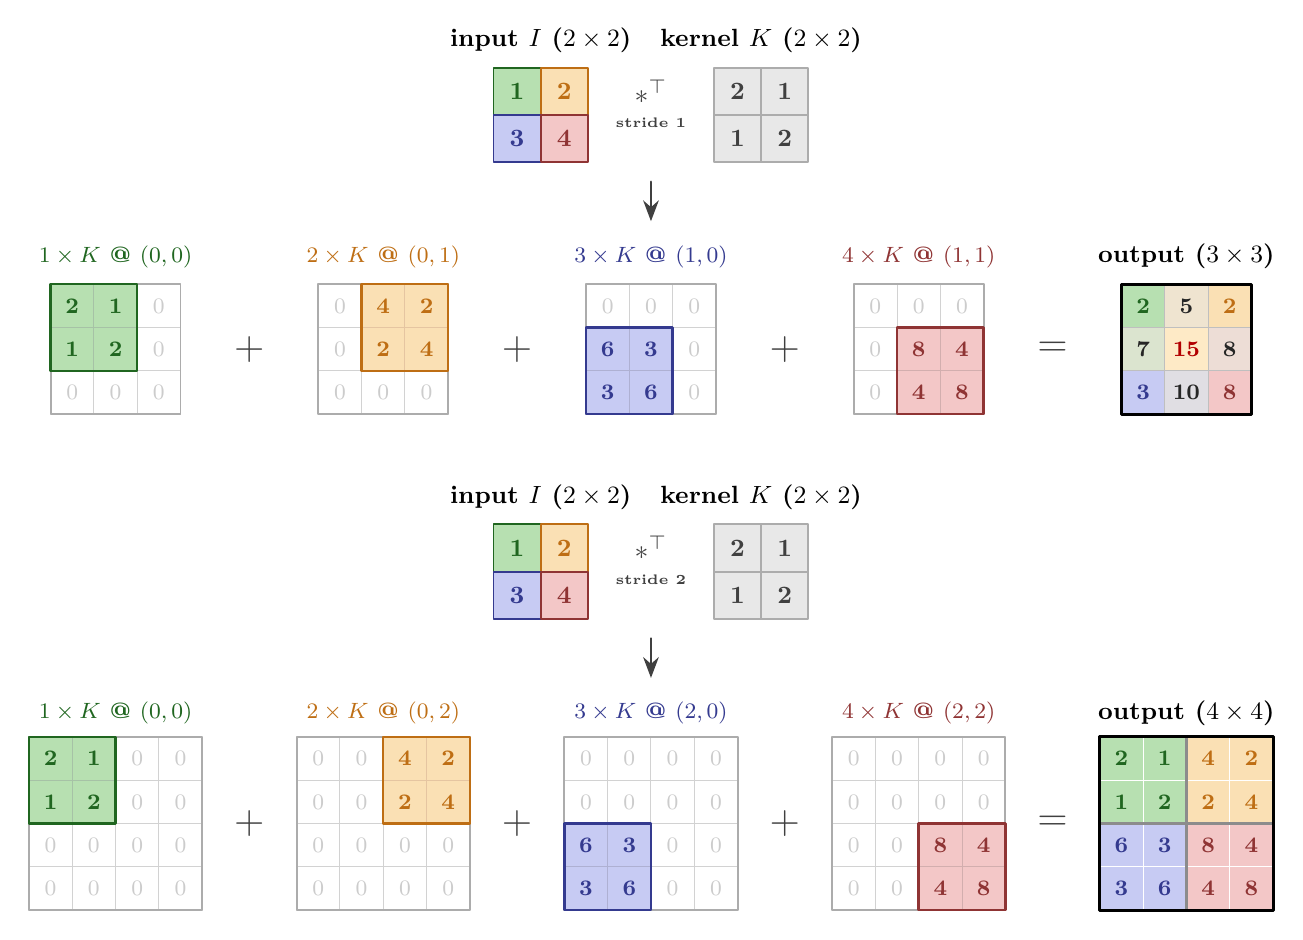
\begin{tikzpicture}[
    font=\small, line join=round, line cap=round,
    every node/.style={inner sep=0pt, outer sep=0pt, align=center},
    arr/.style={->, >=Stealth, line width=.85pt}
  ]

  % =========================================================================
  % 宏定义
  % =========================================================================
  % 3x3 底网格宏 (每个网格 0.55 x 0.55)
  \newcommand{\basegridThree}[2]{%
    \draw[step=.55, gray!35, line width=.35pt, shift={(#1,#2)}] (0,0) grid (1.65,1.65);
    \draw[gray!65, line width=.7pt] (#1,#2) rectangle ++(1.65,1.65);
    \foreach \i in {0,...,2} \foreach \j in {0,...,2}
      \node[font=\footnotesize, text=gray!40] at ({#1+.275+.55*\j},{#2+1.375-.55*\i}) {0};
  }

  % 3x3 画布上的 2x2 激活块
  \newcommand{\blkThree}[6]{%
    \pgfmathsetmacro{\bx}{#1+.55*#4}
    \pgfmathsetmacro{\by}{#2+1.65-.55*(#3+2)}
    \fill[#6Fill] (\bx,\by) rectangle ++(1.1,1.1);
    \draw[step=.55, #6Line!40, line width=.35pt, shift={(\bx,\by)}] (0,0) grid (1.1,1.1);
    \draw[#6Line, line width=.9pt] (\bx,\by) rectangle ++(1.1,1.1);
    \foreach \v [count=\m] in {2,1,1,2}{%
      \pgfmathtruncatemacro{\rr}{div(\m-1,2)}%
      \pgfmathtruncatemacro{\cc}{mod(\m-1,2)}%
      \pgfmathtruncatemacro{\vv}{\v*#5}%
      \node[font=\footnotesize\bfseries, text=#6Line] at ({#1+.275+.55*(#4+\cc)},{#2+1.375-.55*(#3+\rr)}) {\vv};
    }%
  }

  % 4x4 底网格宏
  \newcommand{\basegridFour}[2]{%
    \draw[step=.55, gray!35, line width=.35pt, shift={(#1,#2)}] (0,0) grid (2.2,2.2);
    \draw[gray!65, line width=.7pt] (#1,#2) rectangle ++(2.2,2.2);
    \foreach \i in {0,...,3} \foreach \j in {0,...,3}
      \node[font=\footnotesize, text=gray!40] at ({#1+.275+.55*\j},{#2+1.925-.55*\i}) {0};
  }

  % 4x4 画布上的 2x2 激活块
  \newcommand{\blkFour}[6]{%
    \pgfmathsetmacro{\bx}{#1+.55*#4}
    \pgfmathsetmacro{\by}{#2+2.2-.55*(#3+2)}
    \fill[#6Fill] (\bx,\by) rectangle ++(1.1,1.1);
    \draw[step=.55, #6Line!40, line width=.35pt, shift={(\bx,\by)}] (0,0) grid (1.1,1.1);
    \draw[#6Line, line width=.9pt] (\bx,\by) rectangle ++(1.1,1.1);
    \foreach \v [count=\m] in {2,1,1,2}{%
      \pgfmathtruncatemacro{\rr}{div(\m-1,2)}%
      \pgfmathtruncatemacro{\cc}{mod(\m-1,2)}%
      \pgfmathtruncatemacro{\vv}{\v*#5}%
      \node[font=\footnotesize\bfseries, text=#6Line] at ({#1+.275+.55*(#4+\cc)},{#2+1.925-.55*(#3+\rr)}) {\vv};
    }%
  }

  % =========================================================================
  % 【上半部分】：步长 stride = 1 (有重叠 overlap, 输出 3x3)
  % 间距调整：原 shift={(0, 9.5)} 缩减至 shift={(0, 8.7)}，间距减半
  % =========================================================================
  \begin{scope}[shift={(0, 8.7)}]
    % 1. 顶部：输入 I 与 卷积核 K (水平居中于 x = 7.9)
    \begin{scope}[shift={(7.9, 5.0)}]
      % input I
      \node[font=\small\bfseries] at (-1.4, 0.95) {input \(I\) (\(2\times 2\))};
      \foreach \v/\c [count=\m] in {1/in, 2/or, 3/hid, 4/out}{%
        \pgfmathtruncatemacro{\rr}{div(\m-1,2)}%
        \pgfmathtruncatemacro{\cc}{mod(\m-1,2)}%
        \fill[\c Fill, draw=\c Line, line width=.7pt]
          ({-2.0+.6*\cc},{0.6-.6*(\rr+1)}) rectangle ++(.6,.6);
        \node[font=\small\bfseries, text=\c Line]
          at ({-2.0+.3+.6*\cc},{0.6-.3-.6*\rr}) {\v};
      }

      % 转置卷积符号
      \node[font=\normalsize\bfseries, text=darkgray] at (0, 0.3) {\(\ast^{\top}\)};
      \node[font=\tiny\bfseries, text=darkgray] at (0, -0.1) {stride 1};

      % kernel K
      \node[font=\small\bfseries] at (1.4, 0.95) {kernel \(K\) (\(2\times 2\))};
      \foreach \v [count=\m] in {2,1,1,2}{%
        \pgfmathtruncatemacro{\rr}{div(\m-1,2)}%
        \pgfmathtruncatemacro{\cc}{mod(\m-1,2)}%
        \fill[gray!18, draw=gray!65, line width=.7pt]
          ({0.8+.6*\cc},{0.6-.6*(\rr+1)}) rectangle ++(.6,.6);
        \node[font=\small\bfseries, text=black!75]
          at ({0.8+.3+.6*\cc},{0.6-.3-.6*\rr}) {\v};
      }
    \end{scope}

    % 顶底过渡箭头 (长度 0.5cm)
    \draw[arr, line width=1pt, darkgray] (7.9, 4.15) -- (7.9, 3.65);

    % 2. 四张 3x3 散布画布 (中心 x 严格对齐下方：1.1, 4.5, 7.9, 11.3, 14.7)
    % 分支 1: 1 x K @ (0,0)
    \node[font=\footnotesize\bfseries, text=inLine] at (1.1, 3.2) {\(1\times K\) @ \((0,0)\)};
    \basegridThree{0.275}{1.2}
    \blkThree{0.275}{1.2}{0}{0}{1}{in}
    \node[font=\Large\bfseries, text=darkgray] at (2.8, 2.025) {\(+\)};

    % 分支 2: 2 x K @ (0,1)
    \node[font=\footnotesize\bfseries, text=orLine] at (4.5, 3.2) {\(2\times K\) @ \((0,1)\)};
    \basegridThree{3.675}{1.2}
    \blkThree{3.675}{1.2}{0}{1}{2}{or}
    \node[font=\Large\bfseries, text=darkgray] at (6.2, 2.025) {\(+\)};

    % 分支 3: 3 x K @ (1,0)
    \node[font=\footnotesize\bfseries, text=hidLine] at (7.9, 3.2) {\(3\times K\) @ \((1,0)\)};
    \basegridThree{7.075}{1.2}
    \blkThree{7.075}{1.2}{1}{0}{3}{hid}
    \node[font=\Large\bfseries, text=darkgray] at (9.6, 2.025) {\(+\)};

    % 分支 4: 4 x K @ (1,1)
    \node[font=\footnotesize\bfseries, text=outLine] at (11.3, 3.2) {\(4\times K\) @ \((1,1)\)};
    \basegridThree{10.475}{1.2}
    \blkThree{10.475}{1.2}{1}{1}{4}{out}
    \node[font=\Large\bfseries, text=darkgray] at (13.0, 2.025) {\(=\)};

    % 3. 右侧：最终叠加输出 3x3 (含重叠相加数值)
    \node[font=\small\bfseries] at (14.7, 3.2) {output (\(3\times 3\))};
    \begin{scope}[shift={(13.875, 1.2)}]
      % 各像元底色 (四个角保持对应类色，重叠交界处浅色融合)
      \fill[inFill] (0, 1.1) rectangle ++(0.55, 0.55);
      \fill[mixFill!70!orFill] (0.55, 1.1) rectangle ++(0.55, 0.55);
      \fill[orFill] (1.1, 1.1) rectangle ++(0.55, 0.55);

      \fill[mixFill!70!inFill] (0, 0.55) rectangle ++(0.55, 0.55);
      \fill[yellow!25!orange!20] (0.55, 0.55) rectangle ++(0.55, 0.55);
      \fill[mixFill!70!outFill] (1.1, 0.55) rectangle ++(0.55, 0.55);

      \fill[hidFill] (0, 0) rectangle ++(0.55, 0.55);
      \fill[mixFill!70!hidFill] (0.55, 0) rectangle ++(0.55, 0.55);
      \fill[outFill] (1.1, 0) rectangle ++(0.55, 0.55);

      % 网格线与黑色外边框
      \draw[step=.55, gray!50, line width=.4pt] (0,0) grid (1.65, 1.65);
      \draw[black, line width=1.1pt] (0,0) rectangle (1.65, 1.65);

      % 累加计算值
      \node[font=\footnotesize\bfseries, text=inLine] at (0.275, 1.375) {2};
      \node[font=\footnotesize\bfseries, text=black!85] at (0.825, 1.375) {5};
      \node[font=\footnotesize\bfseries, text=orLine] at (1.375, 1.375) {2};

      \node[font=\footnotesize\bfseries, text=black!85] at (0.275, 0.825) {7};
      \node[font=\footnotesize\bfseries, text=red!70!black] at (0.825, 0.825) {15};
      \node[font=\footnotesize\bfseries, text=black!85] at (1.375, 0.825) {8};

      \node[font=\footnotesize\bfseries, text=hidLine] at (0.275, 0.275) {3};
      \node[font=\footnotesize\bfseries, text=black!85] at (0.825, 0.275) {10};
      \node[font=\footnotesize\bfseries, text=outLine] at (1.375, 0.275) {8};
    \end{scope}
  \end{scope}


  % =========================================================================
  % 【下半部分】：步长 stride = 2 (无重叠 no overlap, 输出 4x4)
  % =========================================================================
  \begin{scope}[shift={(0, 0)}]
    % 1. 顶部：输入 I 与 卷积核 K (严格水平居中于 x = 7.9)
    \begin{scope}[shift={(7.9, 7.9)}]
      % input I
      \node[font=\small\bfseries] at (-1.4, 0.95) {input \(I\) (\(2\times 2\))};
      \foreach \v/\c [count=\m] in {1/in, 2/or, 3/hid, 4/out}{%
        \pgfmathtruncatemacro{\rr}{div(\m-1,2)}%
        \pgfmathtruncatemacro{\cc}{mod(\m-1,2)}%
        \fill[\c Fill, draw=\c Line, line width=.7pt]
          ({-2.0+.6*\cc},{0.6-.6*(\rr+1)}) rectangle ++(.6,.6);
        \node[font=\small\bfseries, text=\c Line]
          at ({-2.0+.3+.6*\cc},{0.6-.3-.6*\rr}) {\v};
      }

      % 转置卷积符号
      \node[font=\normalsize\bfseries, text=darkgray] at (0, 0.3) {\(\ast^{\top}\)};
      \node[font=\tiny\bfseries, text=darkgray] at (0, -0.1) {stride 2};

      % kernel K
      \node[font=\small\bfseries] at (1.4, 0.95) {kernel \(K\) (\(2\times 2\))};
      \foreach \v [count=\m] in {2,1,1,2}{%
        \pgfmathtruncatemacro{\rr}{div(\m-1,2)}%
        \pgfmathtruncatemacro{\cc}{mod(\m-1,2)}%
        \fill[gray!18, draw=gray!65, line width=.7pt]
          ({0.8+.6*\cc},{0.6-.6*(\rr+1)}) rectangle ++(.6,.6);
        \node[font=\small\bfseries, text=black!75]
          at ({0.8+.3+.6*\cc},{0.6-.3-.6*\rr}) {\v};
      }
    \end{scope}

    % 顶底过渡箭头 (长度 0.5cm，上下空隙与上面完全一致：0.25cm 与 0.45cm)
    \draw[arr, line width=1pt, darkgray] (7.9, 7.05) -- (7.9, 6.55);

    % 2. 四张 4x4 散布画布
    % 分支 1: 1 x K @ (0,0)
    \node[font=\footnotesize\bfseries, text=inLine] at (1.1, 6.1) {\(1\times K\) @ \((0,0)\)};
    \basegridFour{0}{3.6}
    \blkFour{0}{3.6}{0}{0}{1}{in}
    \node[font=\Large\bfseries, text=darkgray] at (2.8, 4.7) {\(+\)};

    % 分支 2: 2 x K @ (0,2)
    \node[font=\footnotesize\bfseries, text=orLine] at (4.5, 6.1) {\(2\times K\) @ \((0,2)\)};
    \basegridFour{3.4}{3.6}
    \blkFour{3.4}{3.6}{0}{2}{2}{or}
    \node[font=\Large\bfseries, text=darkgray] at (6.2, 4.7) {\(+\)};

    % 分支 3: 3 x K @ (2,0)
    \node[font=\footnotesize\bfseries, text=hidLine] at (7.9, 6.1) {\(3\times K\) @ \((2,0)\)};
    \basegridFour{6.8}{3.6}
    \blkFour{6.8}{3.6}{2}{0}{3}{hid}
    \node[font=\Large\bfseries, text=darkgray] at (9.6, 4.7) {\(+\)};

    % 分支 4: 4 x K @ (2,2)
    \node[font=\footnotesize\bfseries, text=outLine] at (11.3, 6.1) {\(4\times K\) @ \((2,2)\)};
    \basegridFour{10.2}{3.6}
    \blkFour{10.2}{3.6}{2}{2}{4}{out}
    \node[font=\Large\bfseries, text=darkgray] at (13.0, 4.7) {\(=\)};

    % 3. 右侧：最终叠加输出 4x4
    \node[font=\small\bfseries] at (14.7, 6.1) {output (\(4\times 4\))};
    \foreach \v/\c [count=\m] in {
      2/in,  1/in,  4/or,  2/or,
      1/in,  2/in,  2/or,  4/or,
      6/hid, 3/hid, 8/out, 4/out,
      3/hid, 6/hid, 4/out, 8/out}{%
      \pgfmathtruncatemacro{\rr}{div(\m-1,4)}%
      \pgfmathtruncatemacro{\cc}{mod(\m-1,4)}%
      \fill[\c Fill] ({13.6+.55*\cc},{3.6+2.2-.55*(\rr+1)}) rectangle ++(.55,.55);
      \node[font=\footnotesize\bfseries, text=\c Line] at ({13.6+.275+.55*\cc},{3.6+1.925-.55*\rr}) {\v};
    }
    \draw[step=.55, white, line width=.4pt, shift={(13.6,3.6)}] (0,0) grid (2.2,2.2);
    \draw[line width=.85pt, darkgray!60] (14.7, 3.6) -- (14.7, 5.8);
    \draw[line width=.85pt, darkgray!60] (13.6, 4.7) -- (15.8, 4.7);
    \draw[black, line width=1.1pt] (13.6,3.6) rectangle ++(2.2,2.2);
  \end{scope}

\end{tikzpicture}
\end{document}